\section{Method}
\label{sec:method}

\subsection{Problem formulation and input design}
\label{sec:formulation}

We formulate battery prognostics as a sliding-window capacity
forecasting problem. Let $c_t$ denote the measured capacity at cycle
$t$. Given a fixed-length input window
$\mathbf{X}_{t} = [c_{t-W+1}, \ldots, c_t]$ of historical capacity,
the model predicts future capacity values. The main model
deliberately consumes \emph{capacity only}, for a deployment-driven
reason: at inference, the future values of voltage, current,
temperature, and internal resistance are unavailable, so any model
consuming them cannot be rolled out autoregressively to the end of
life without information leakage. Capacity is the only health
indicator that is both measurable online and self-contained for
rollout. The physics-consistent extension of
Section~\ref{sec:physics} additionally consumes the per-cycle
\emph{measured} internal resistance---a quantity the BMS records in
situ, available at inference without future information---so the
extension remains deployable under the same constraint.

\subsection{Gated DeltaNet-2 backbone}
\label{sec:gdn2}

The backbone is Gated DeltaNet-2 (GDN-2) \cite{ref_gdn2}, a
recurrent linear attention layer with channel-wise erase and write
gates. For one head with key dimension $d_k$ and value dimension
$d_v$, the recurrence is
\begin{equation}
\label{eq:gdn2}
\mathbf{S}_t \;=\; \left( \mathbf{I} - \mathbf{k}_t(\mathbf{b}_t
\odot \mathbf{k}_t)^{\top} \right)
\operatorname{diag}(\boldsymbol{\alpha}_t)\, \mathbf{S}_{t-1}
\;+\; \mathbf{k}_t(\mathbf{w}_t \odot \mathbf{v}_t)^{\top},
\end{equation}
\begin{equation}
\label{eq:readout}
\mathbf{o}_t \;=\; \mathbf{S}_t^{\top}\mathbf{q}_t,
\end{equation}
where $\mathbf{q}_t,\mathbf{k}_t \in \mathbb{R}^{d_k}$ and
$\mathbf{v}_t \in \mathbb{R}^{d_v}$ are query, key, and value vectors;
$\mathbf{b}_t \in \mathbb{R}^{d_k}$ is the channel-wise erase gate and
$\mathbf{w}_t \in \mathbb{R}^{d_v}$ the channel-wise write gate, both
bounded to $[0,1]$ by a sigmoid; and
$\boldsymbol{\alpha}_t = \exp(\mathbf{g}_t)$ is the channel-wise decay
with
\begin{equation}
\mathbf{g}_t \;=\; -A_{\log}\cdot
\operatorname{softplus}\!\big( f(\mathbf{x}_t) + \mathbf{d}_t \big),
\end{equation}
where $\mathbf{x}_t$ is the input token at position $t$ (the embedded
capacity, or the branch's hidden representation after the first
layer), $A_{\log}$ is a per-head log-rate, $f(\cdot)$ a two-layer
projection, and $\mathbf{d}_t$ a per-channel bias. The state
$\mathbf{S}_t \in \mathbb{R}^{d_k \times d_v}$ is fixed-size and
updated incrementally, yielding $O(N)$ scan complexity with
constant memory. With $H$ heads, $d_k=16$, and $d_v=32$, the total
state is $H \cdot d_k \cdot d_v \cdot 4$ bytes $= 8$\,KB per layer.
Figure~\ref{fig:evidence}\subref{fig:cost} contrasts the per-window cost of this
scan with quadratic self-attention.
During a window scan the state is updated incrementally---each new
cycle erases part of the old memory (via $\mathbf{b}_t$) and writes
new information (via $\mathbf{w}_t$)---so the fixed-size matrix acts
as an adaptive compression of the degradation history rather than a
static buffer.

\subsection{Multi-scale branches with per-layer cross-scale exchange}
\label{sec:multiscale}

Figure~\ref{fig:arch} shows the multi-scale encoder
together with the per-layer cross-scale exchange submodule (bottom,
light-green box), and Figure~\ref{fig:gdn2} details the internal
recurrence of one GDN-2 block.

\begin{figure}[!ht]
\centering
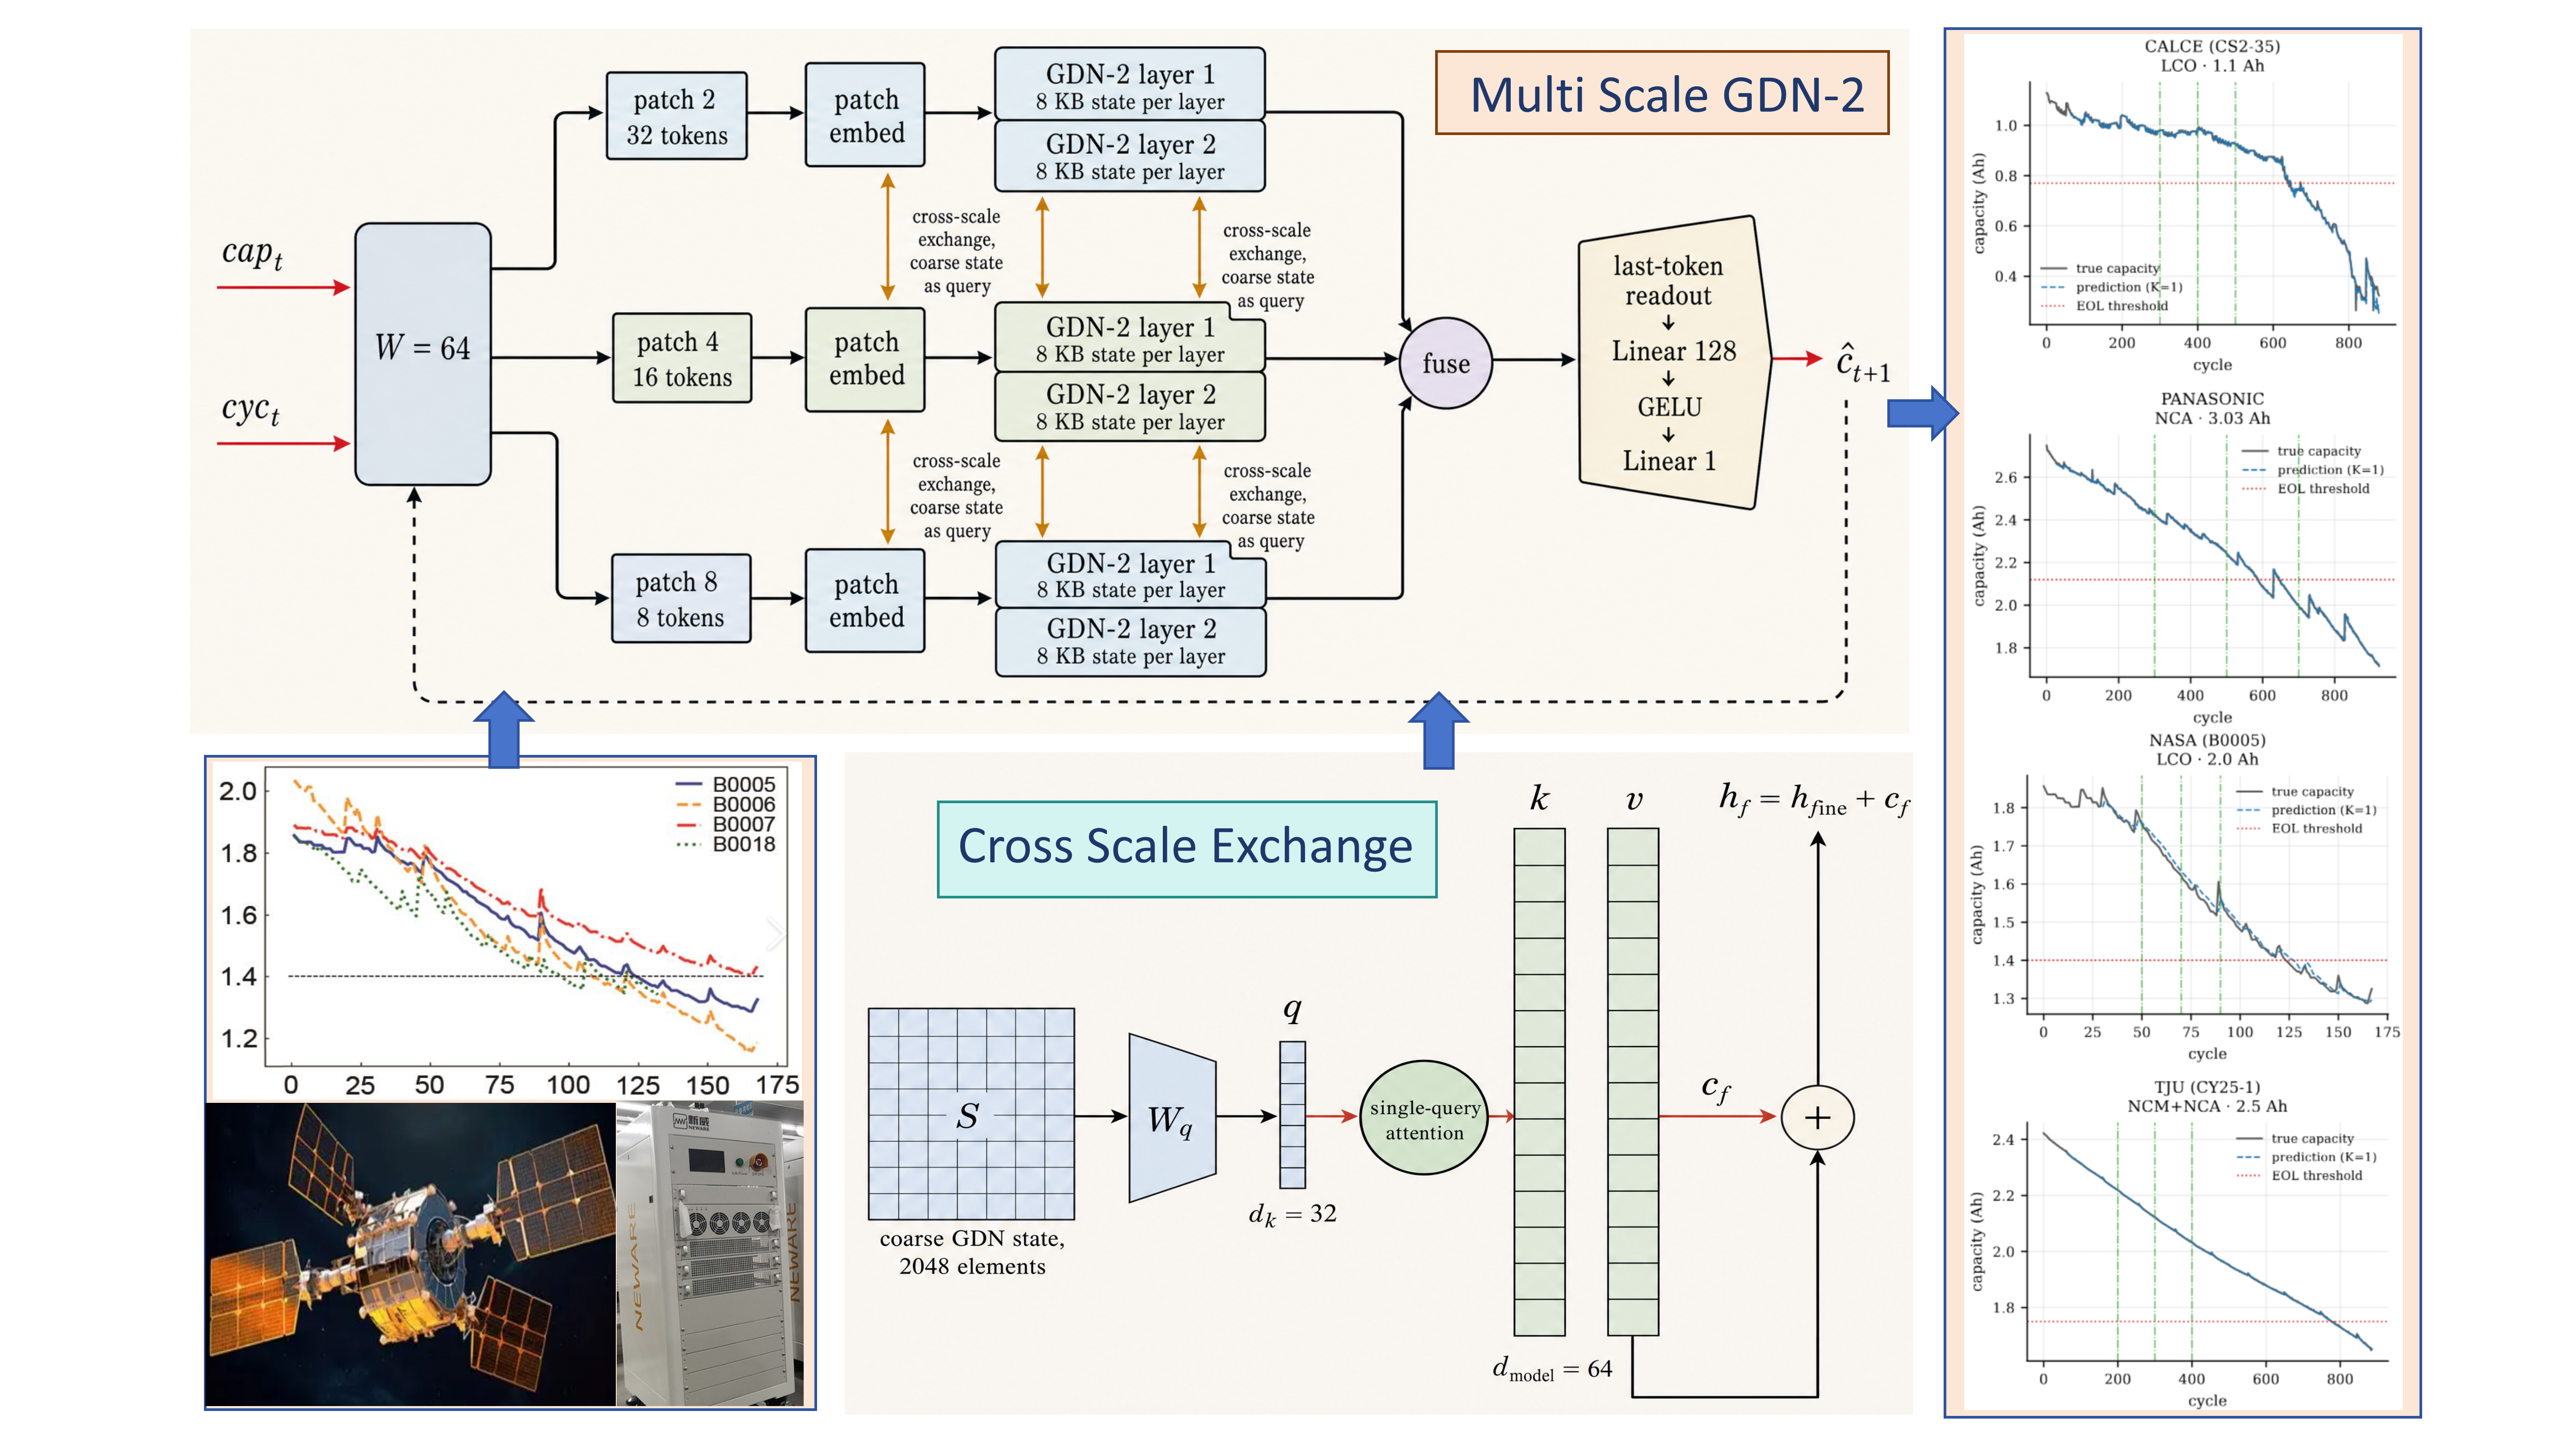
\includegraphics[width=\textwidth]{figures/new_modelarch.png}
\caption{Multi-scale GDN-2 architecture and cross-scale exchange
submodule. Top: the fixed window of $W{=}64$ capacity cycles (the
tokens $cap_t$; $cyc_t$ denotes the cycle index) is encoded in
parallel at three scales (patch 2/4/8, 32/16/8 tokens), embedded
per scale, and passed through two GDN-2 layers per branch ($8$\,KB
fixed state per layer); the three branches exchange multi-scale
information through the per-layer cross-scale exchange (orange
arrows, coarse state as query), fuse at the $fuse$ node, and emit
the next-cycle capacity prediction
$\hat{c}_{t+1}$ via the last-token readout (Linear\,128 $\to$ GELU
$\to$ Linear\,1). Bottom (light-green box): the cross-scale exchange
submodule maps the coarse state $S$ (2048 elements) to a single
query $q$ ($d_q{=}32$) via $W_q$; single-query attention interacts
$q$ with the fine/mid branch keys and values ($k, v$,
$d_{\text{model}}{=}64$) to produce the context $c_f$, added to the
fused state: $h_f = h_{\text{fuse}} + c_f$.}
\label{fig:arch}
\end{figure}

\begin{figure}[!ht]
\centering
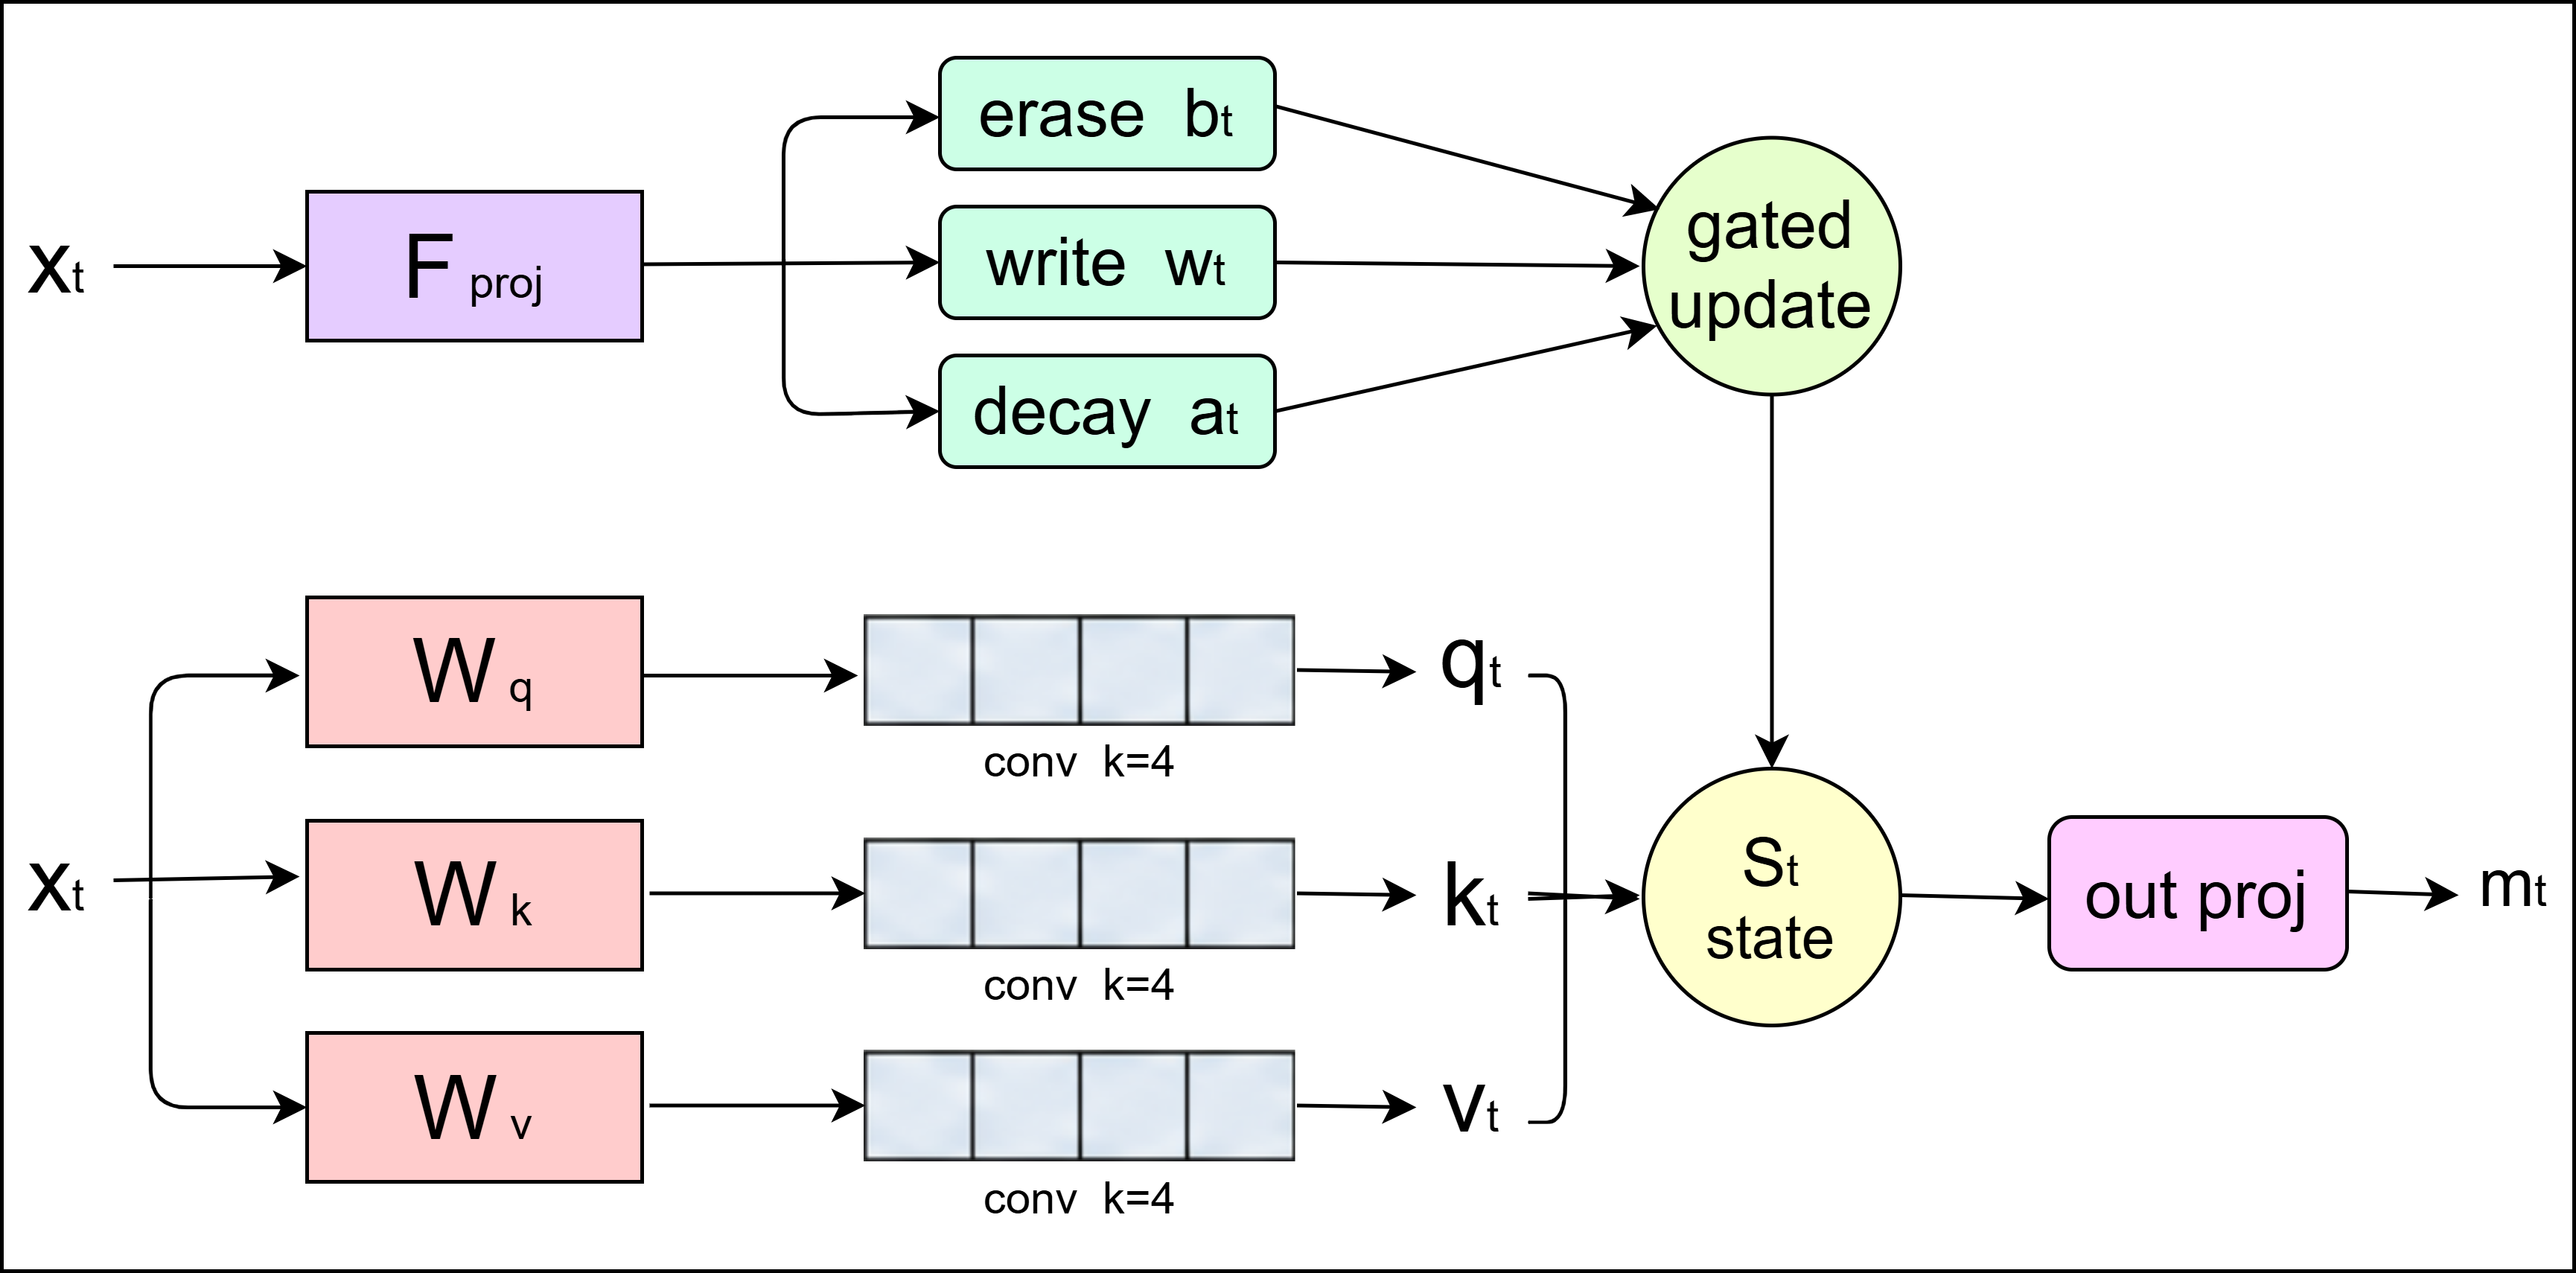
\includegraphics[width=0.85\textwidth]{figures/fig_gdn2_flow}
\caption{One GDN-2 block. The input token $x_t$ is projected to
queries/keys/values ($W_q$: $64\to64$, $W_k$: $64\to64$,
$W_v$: $64\to128$), each through a causal 1-D convolution
(kernel $k{=}4$, $L2$-normalized for $q$ and $k$), while a shared
projection $F_{\mathrm{proj}}$ generates the erase
($\mathbf{b}_t$, sigmoid), write ($\mathbf{w}_t$, sigmoid) and
per-channel decay ($\boldsymbol{\alpha}_t = \exp(g)$) gates; the
gated update produces the fixed-size state
$\mathbf{S}_t$ ($4\times16\times32$ elements $= 8$\,KB, zero
growth), and the output
$\mathbf{o}_t = \mathbf{S}_t^{\top}\mathbf{q}_t \to$ Linear
$128\to64 \to$ RMSNorm.
}
\label{fig:gdn2}
\end{figure}

\begin{figure}[!ht]
\centering
\begin{subfigure}[b]{0.32\textwidth}
\centering
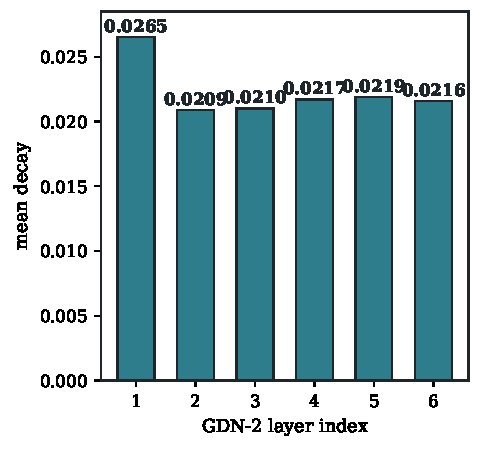
\includegraphics[width=\linewidth]{figures/fig_evidence_decay}
\caption{}
\label{fig:decay}
\end{subfigure}\hfill
\begin{subfigure}[b]{0.32\textwidth}
\centering
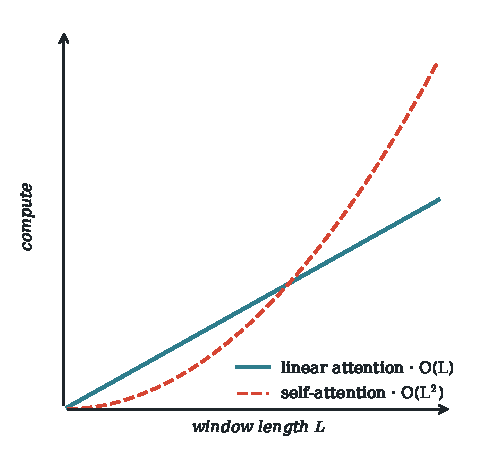
\includegraphics[width=\linewidth]{figures/fig_evidence_complexity}
\caption{}
\label{fig:cost}
\end{subfigure}\hfill
\begin{subfigure}[b]{0.32\textwidth}
\centering
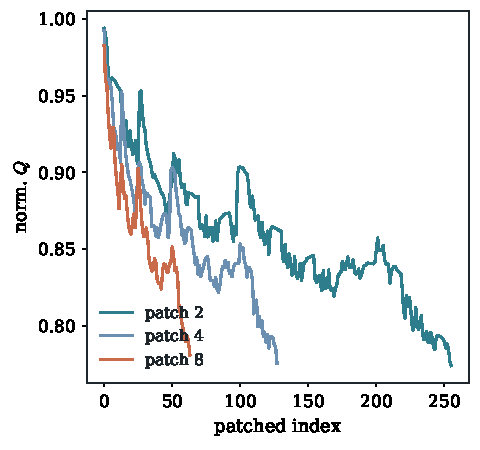
\includegraphics[width=\linewidth]{figures/fig_evidence_patch}
\caption{}
\label{fig:patch_pool}
\end{subfigure}
\caption{Method-consistency evidence. (a) Real per-layer mean decay
weights from the seed-42 CALCE checkpoint: each layer keeps state
over hundreds of cycles, and the per-channel log-rate gate
($g = -\exp(A_{\log})\,\mathrm{softplus}(\mathrm{raw}_g +
\mathrm{dt}_{\mathrm{bias}})$, $\boldsymbol{\alpha}_t=\exp(g)$)
sets how quickly each channel forgets. (b) Per-window cost of the
single-query linear-attention scan ($O(L)$) versus quadratic
self-attention ($O(L^2)$). (c) Real multi-scale capacity series of
the $W{=}64$ CALCE window under patch sizes $P\in\{2,4,8\}$
(32/16/8 tokens).}
\label{fig:evidence}
\end{figure}

Battery degradation operates across multiple temporal scales: short
regeneration events, mid-range knee-point transitions, and the
long-term monotonic envelope. We encode these with three parallel
branches using patch sizes $P \in \{2,4,8\}$
(Figure~
ef{fig:evidence}\subref{fig:patch_pool} shows the real capacity series at each
patch scale). Each branch projects its
patched input to a common $d_{\text{model}}=64$ embedding and applies
two GDN-2 layers. After every GDN layer, branches exchange
information through a stage-query mechanism: the coarse branch's
GDN-2 state---the compressed degradation history, which acts as a
stage indicator---is projected to a single query, and the fine and
mid branch sequences provide keys and values. For branch
$\mathbf{h}_a$ with the coarse state $\mathbf{S}_c$,
\begin{equation}
\label{eq:stagequery}
\mathbf{q} \;=\; \mathbf{W}_q \operatorname{vec}(\mathbf{S}_c),
\qquad
\mathbf{h}_a' \;=\; \mathbf{h}_a \;+\;
\sum_{t} \frac{\exp\!\big(\mathbf{k}_t^{\top}\mathbf{q}/\sqrt{d_k}\big)}
{\sum_{s} \exp\!\big(\mathbf{k}_s^{\top}\mathbf{q}/\sqrt{d_k}\big)}
\,\mathbf{v}_t,
\end{equation}
where $\mathbf{k}_t = \mathbf{W}_k \mathbf{h}_a[t]$ and
$\mathbf{v}_t = \mathbf{W}_v \mathbf{h}_a[t]$, and the summation is a
single-query linear-attention readout with $O(L)$ cost per layer.
The exchange is additive (residual, no gating) and applied
per layer. Ablation studies (Section \ref{sec:ablation}) show that
branches without interaction degrade consistently (CALCE MAE $0.0068$ vs $0.0065$; Wilcoxon $p=0.037$), while the stage-query exchange restores the multi-scale model to the single-branch level on CALCE and yields the best mean on the regeneration-rich NASA dataset ($0.0084$ vs $0.0087$); the exchange never degrades accuracy relative to a single branch.

An interpretability analysis (Section \ref{sec:phys}) reveals that
the coarse branch (patch 8) spontaneously encodes the degradation
stage: its pooled representation is $93.2\%$ linearly separable into
early/mid/late life stages on the PANASONIC dataset ($2.9\times$
chance), providing stage-aware state awareness at no additional
supervision cost.

\subsection{Physics-consistent extension: the rate head}
\label{sec:physics}

The main architecture of Section~\ref{sec:multiscale} is trained
purely data-driven under the baseline-consistent per-window protocol.
Here we present a physics-consistent extension whose design is the
outcome of a systematic injection-route study (Section
\ref{sec:phys}): a degradation-rate head driven by a measured
physical feature. Lithium-ion capacity fade is governed by
thermally activated processes---solid-electrolyte-interface growth,
loss of lithium inventory, and active-material loss---and internal
resistance (IR) is a direct, independently measured observable of
these aging processes that rises as the cell degrades. We therefore
decompose the per-cycle decay rate into a learned component and a
physics-feature component:
\begin{equation}
\label{eq:rate_head}
r \;=\; \operatorname{softplus}(\mathbf{w}^{\top}\mathbf{h})
\;+\; \operatorname{softplus}(\gamma)\cdot \mathrm{IR}_{\text{last}},
\qquad
\hat{c}_{t+1} \;=\; c_t - r,
\end{equation}
where $\mathbf{h}$ is the last-token GDN state, $c_t$ the current
capacity, and $\mathrm{IR}_{\text{last}}$ the measured internal
resistance at the current cycle. The softplus constraint makes
$\gamma \ge 0$: internal-resistance growth can only \emph{accelerate}
decay, never decelerate it---the physical direction of SEI-driven
aging. The formulation is structurally monotonic
($\hat{c}_{t+1} \le c_t$) and therefore cannot emit nonphysical
regeneration artifacts by construction.

The rate head is trained in \emph{absolute} capacity space
($\mathcal{L} = \operatorname{MAE}(\hat{c}, c)$) rather than the
per-window z-score protocol: z-score targets include positive values
(plateau segments where the next observation lies above the window
mean) that a monotone predictor can never produce, so the constraint
is unsatisfiable in that space; the absolute-space objective removes
the sign conflict. A control experiment confirms the mechanism, not
the objective, is responsible for the gain: a free head trained in
absolute space reaches MAE $0.0097$ (worse than the z-score free head
at $0.0070$), while the rate head reaches $0.0042$. The extension
further improves the unseen-tail extrapolation ($R^2$ $0.775$ vs
$0.374$) and robustness to corrupted inputs (Section
\ref{sec:ablation}).

\subsection{Readout and training protocol}
\label{sec:readout}

After the multi-scale encoder, the fused last-token representation
$\mathbf{h}_{t}$ is passed through a readout
\begin{equation}
\label{eq:head}
\hat{c}_{t+1}
\;=\; \operatorname{Head}(\mathbf{h}_t)
\;=\; \mathbf{W}_2\, \mathrm{GELU}(\mathbf{W}_1 \mathbf{h}_t),
\end{equation}
with $d = 3 \cdot d_{\text{model}} = 192$ the dimension of the fused
last-token representation (concatenation of the three branches),
$\mathbf{W}_1 \in \mathbb{R}^{128 \times d}$ and
$\mathbf{W}_2 \in \mathbb{R}^{1 \times 128}$. The model is trained
with the per-window z-score target protocol of PatchFormer and
RUL-Mamba for baseline comparability: the input window is normalized
globally with training-cell min--max statistics, the target is
$(c_{t+1} - \bar{c})/\sigma_c$ with window statistics
$(\bar{c}, \sigma_c)$, and predictions are de-normalized with the
same window statistics at evaluation.

\subsection{Uncertainty quantification with conformal calibration}
\label{sec:quantile}

Safety-critical BMS decisions require not only a point estimate of
the health state but a calibrated interval, e.g., ``the cell will
cross the EOL threshold within 30--50 cycles with 95\% confidence''.
To provide this without the cost of an ensemble, the readout head
outputs three quantiles per forward pass,
$q \in \{0.025, 0.5, 0.975\}$ (P2.5, the median P50, and P97.5),
bounding a central 95\% interval. The head is trained
with the pinball (quantile) loss
\begin{equation}
\mathcal{L}_{\text{pin}} \;=\;
\frac{1}{N}\sum_{i}\sum_{q \in \{0.025,0.5,0.975\}}
\rho_q\!\left( c_i - \hat{c}_i^{(q)} \right),
\qquad
\rho_q(u) = \max(q u, (q-1) u),
\end{equation}
where $c_i$ is the observed capacity, $\hat{c}_i^{(q)}$ is the
predicted $q$-quantile, and the pinball function $\rho_q$ penalizes
under-prediction (when $\hat{c}^{(q)} > c$) by a factor $q$ and
over-prediction by $1-q$, so that the minimizer is the conditional
$q$-quantile. Because a lower capacity trajectory crosses the EOL
threshold earlier, P2.5 yields the \emph{earliest} plausible EOL
crossing and P97.5 the \emph{latest}; the P2.5--P97.5 crossing
window is therefore a safety-relevant interval (the pessimistic
bound drives maintenance scheduling).

Quantile regression alone is known to be miscalibrated under
distribution shift. We therefore apply \emph{conformalized quantile
regression} (CQR): a held-out calibration cell provides conformity
scores $s_i = \max(\hat{c}_i^{\text{lo}} - c_i,\; c_i -
\hat{c}_i^{\text{hi}})$, and the deployed interval is inflated by
$q_{\text{adj}}$, the $(1-\alpha)(1+1/n)$ empirical quantile of the
scores, where $\alpha = 0.05$ and $n$ is the calibration size.
Calibration and coverage results are reported in
Section~\ref{sec:conf}. The entire UQ mechanism costs one forward
pass and two scalars at deployment---no ensemble, no MC sampling.

